%%
%% Automatically generated file from DocOnce source
%% (https://github.com/doconce/doconce/)
%% doconce format latex final.do.txt --no_mako
%%
% #ifdef PTEX2TEX_EXPLANATION
%%
%% The file follows the ptex2tex extended LaTeX format, see
%% ptex2tex: https://code.google.com/p/ptex2tex/
%%
%% Run
%%      ptex2tex myfile
%% or
%%      doconce ptex2tex myfile
%%
%% to turn myfile.p.tex into an ordinary LaTeX file myfile.tex.
%% (The ptex2tex program: https://code.google.com/p/ptex2tex)
%% Many preprocess options can be added to ptex2tex or doconce ptex2tex
%%
%%      ptex2tex -DMINTED myfile
%%      doconce ptex2tex myfile envir=minted
%%
%% ptex2tex will typeset code environments according to a global or local
%% .ptex2tex.cfg configure file. doconce ptex2tex will typeset code
%% according to options on the command line (just type doconce ptex2tex to
%% see examples). If doconce ptex2tex has envir=minted, it enables the
%% minted style without needing -DMINTED.
% #endif

% #define PREAMBLE

% #ifdef PREAMBLE
%-------------------- begin preamble ----------------------

\documentclass[%
oneside,                 % oneside: electronic viewing, twoside: printing
final,                   % draft: marks overfull hboxes, figures with paths
10pt]{article}

\listfiles               %  print all files needed to compile this document

\usepackage{relsize,makeidx,color,setspace,amsmath,amsfonts,amssymb}
\usepackage[table]{xcolor}
\usepackage{bm,ltablex,microtype}

\usepackage[pdftex]{graphicx}

\usepackage[T1]{fontenc}
%\usepackage[latin1]{inputenc}
\usepackage{ucs}
\usepackage[utf8x]{inputenc}

\usepackage{lmodern}         % Latin Modern fonts derived from Computer Modern

% Hyperlinks in PDF:
\definecolor{linkcolor}{rgb}{0,0,0.4}
\usepackage{hyperref}
\hypersetup{
    breaklinks=true,
    colorlinks=true,
    linkcolor=linkcolor,
    urlcolor=linkcolor,
    citecolor=black,
    filecolor=black,
    %filecolor=blue,
    pdfmenubar=true,
    pdftoolbar=true,
    bookmarksdepth=3   % Uncomment (and tweak) for PDF bookmarks with more levels than the TOC
    }
%\hyperbaseurl{}   % hyperlinks are relative to this root

\setcounter{tocdepth}{2}  % levels in table of contents

% Tricks for having figures close to where they are defined:
% 1. define less restrictive rules for where to put figures
\setcounter{topnumber}{2}
\setcounter{bottomnumber}{2}
\setcounter{totalnumber}{4}
\renewcommand{\topfraction}{0.95}
\renewcommand{\bottomfraction}{0.95}
\renewcommand{\textfraction}{0}
\renewcommand{\floatpagefraction}{0.75}
% floatpagefraction must always be less than topfraction!
% 2. ensure all figures are flushed before next section
\usepackage[section]{placeins}
% 3. enable begin{figure}[H] (often leads to ugly pagebreaks)
%\usepackage{float}\restylefloat{figure}

% prevent orhpans and widows
\clubpenalty = 10000
\widowpenalty = 10000

% --- end of standard preamble for documents ---


% insert custom LaTeX commands...

\raggedbottom
\makeindex
\usepackage[totoc]{idxlayout}   % for index in the toc
\usepackage[nottoc]{tocbibind}  % for references/bibliography in the toc

%-------------------- end preamble ----------------------

\begin{document}

% matching end for #ifdef PREAMBLE
% #endif

\newcommand{\exercisesection}[1]{\subsection*{#1}}


% ------------------- main content ----------------------



% ----------------- title -------------------------

\thispagestyle{empty}

\begin{center}
{\LARGE\bf
\begin{spacing}{1.25}
PHY321 Classical Mechanics 1
\end{spacing}
}
\end{center}

% ----------------- author(s) -------------------------

\begin{center}
{\bf Final  project Spring semester 2023, due Friday May 5}
\end{center}

    \begin{center}
% List of all institutions:
\centerline{{\small midnight (1159pm)}}
\end{center}
    
% ----------------- end author(s) -------------------------

% --- begin date ---
\begin{center}
April 26, 2023
\end{center}
% --- end date ---

\vspace{1cm}


\subsection{Practicalities about  homeworks and projects (midterms and final)}

\begin{enumerate}
\item You can work in groups (optimal groups are often 2-3 people) or by yourself. If you work as a group you can hand in one answer only if you wish. \textbf{Remember to write your name(s)}!

\item How do I(we)  hand in?  Due to the extraordinary situation we are in now, the final projec should be handed in fully via D2L. You can scan your handwritten notes and upload to D2L or you can hand in everyhting (if you are ok with typing mathematical formulae using say Latex) as a jupyter notebook at D2L. The numerical part should always be handed in as a jupyter notebook.
\end{enumerate}

\noindent
\paragraph{Introduction to the final project, total score: 160  points.}
The relevant reading background is
\begin{enumerate}
\item Chapters 2-8 and 14 of Taylor

\item Lecture notes throughout the semester and homework assignments and midterm projects.
\end{enumerate}

\noindent
\paragraph{Exercise 1, motion of a balloon (75pt).}
This exercise brings us back to the beginning of the semester and
homework assignments 2 and 3, in particular exercises 5 and 6 of
homework 3. The relevant chapter of Taylor's text is chapter 2 and
partly chapter 3. The code you wrote for homework 3 may be useful.

In this exercise we will develop a model to determine the motion of a
weather balloon released from the ground. We start from a simplified
model and gradually add features to make our model more realistic.

After the balloon is released, it is driven by buoyancy. Initially, we will assume that the buoyancy force is given by a constant force, $\bm{B}$.
We assume that the motion is vertical only and label this in terms of the $z$-axis.  That is our system is one-dimensional only.
The constant buoyancy force is then given by its $z$-component only, that is $\bm{B}=B_z\bm{k}$, where $\bm{k}$ is the unit vector along the $z$-axis.
\begin{itemize}
\item \textbf{1a (5pt)}: Draw a diagram of the balloon and identify and label the forces. 

\item \textbf{1b (5pt)}: We neglect air resistance here. What is the acceleration of the balloon?

\item \textbf{1c (5pt)}: Find the position and velocity of the balloon as a function of time.
\end{itemize}

\noindent
Let us now introduce air resistance, using a quadratic law: $\bm{F}_D
= −D \vert \bm{v}\vert \bm{v}$, where $D$ is a constant and $\bm{v}$
is the velocity. We are still in one dimension but have introduced
forces and velocities as vectors (boldfaced quantities).

\begin{itemize}
\item \textbf{1d (5pt):} Show that the acceleration of the balloon in the upward $z$ direction is $a_z = (B_z/m)−g−(D/m)|v_z|v_z$,where $v_z$ is the velocity in the $z$-direction.

\item \textbf{1e (5pt):} Find the asymptotic (terminal) velocity of the balloon. Sketch the acceleration and velocity as a function of time for the model including air resistance and define the initial conditions.
\end{itemize}

\noindent
The balloon is released on a windy day, with a wind blowing with a velocity
given by $\bm{w} = w_x \bm{i}$ along the horizontal $x$-axis.

\begin{itemize}
\item \textbf{1f (5pt):} How does the wind modify the air resistance force $\bm{F}_D$ on the balloon?

\item \textbf{1g (5pt):} Draw a diagram of the system (the balloon) in this case and identify and label the forces, as you did in \textbf{1a}.

\item \textbf{1h (5pt):} Find an expression for the acceleration $\bm{a}$ of the balloon. Define the initial conditions for the motion of the balloon.

\item \textbf{1i (5pt):} Why do we call the motion in the $z$ and the $x$ directions as \emph{coupled} in this case? Can you determine the motion of the balloon analytically?

\item \textbf{1j (20pt):} Use now your codes from homework 3 or similar and find the velocity and position of the balloon as functions of time. Plot the position and the velocity with chosen initial conditions and discuss the motion of the balloon. Find the asymptotic (terminal) velocity of the balloon.
\end{itemize}

\noindent
In a real situation, the wind velocity is smaller near the ground and
increases gradually to the full velocity $w_0$ as the balloon moves
upward. Typically, the velocity of the wind as function of the height $z$ can be described
by
\[
\bm{w}(z) = w_0 (1−\exp{(−z/d)}) \bm{i},
\]
where $d = 10$m is a length determining the change in height.

\begin{itemize}
\item \textbf{1k (10pt):} Rewrite your program to include this effect and plot the velocity and position as functions of time. What is the terminal velocity of the balloon now?
\end{itemize}

\noindent
\paragraph{Exercise 2: Mathematical pendulum (85pt).}
A mathematical pendulum consists of a point mass $m$ suspended by a
massless thread/rod of length $l$ in a gravitational field, as shown
in the figure here. The constraining force is labeled by $\bm{T}$ and
the gravitational force is labeled $\bm{F}_g$.  Homework assignments 6 and 7 may be useful to study here. Taylor chapter 5 is the relevant reference for this exercise.

\vspace{6mm}

% inline figure
\centerline{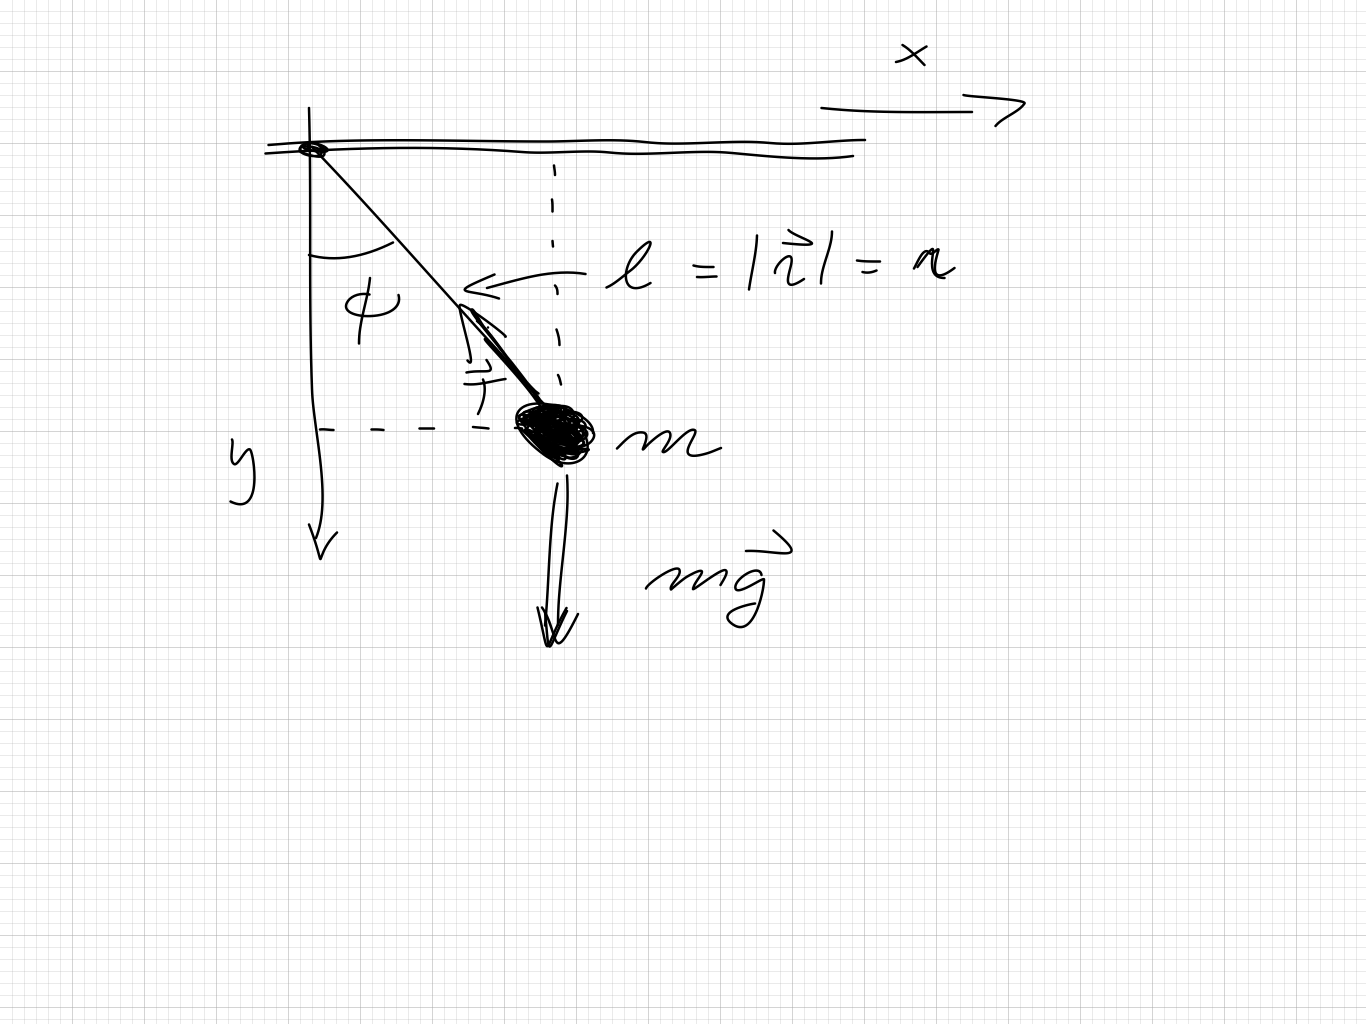
\includegraphics[width=0.6\linewidth]{figures/Simplependulum.png}}

\vspace{6mm}

We assume that the length $l$ is constant and we define the coordinates involved as

\[
\bm{r} = l\sin(\phi)\bm{i}+l\cos(\phi)\bm{j},
\]
where $\bm{i}$ and $\bm{j}$ are the unit vectors in the $x$ and $y$ directions, respectively.

\begin{itemize}
\item \textbf{2a (10pt):} Set up the forces acting on the system and show that the equation of motion is $m\ddot{\bm{r}}=\bm{F}_g+\bm{T}$.
\end{itemize}

\noindent
Transforming to polar coordinates $r$ and $\phi$, 
the equation for $\phi$ is a second-order differential equation (you don't need to show this)
\[
\ddot{\phi}(t)=-\omega_0^2\sin{(\phi(t))}.
\]

This equation can be solved analytically if we assume that the angle $\phi$ is very small. Then we can approximate our equation as

\[
\ddot{\phi}(t)=-\omega_0^2\phi(t).
\]

\begin{itemize}
\item \textbf{2b (10pt):} Find the analytical solution for the last equation. Hint, look back at the solutions for the simple harmonic oscillator problem in one dimension in for example homework 6 and chapter 5 of Taylor.
\end{itemize}

\noindent
For our numerical treatment of the full second-order differential  equation, we can proceed as we have done before and split the second-order differential in two first-order differential equations
as shown here

\[
\frac{d\dot{\phi}}{dt}=-\omega_0^2\sin{(\phi)}.
\]

and

\[
\frac{d\phi}{dt}=\dot{\phi}.
\]

\begin{itemize}
\item \textbf{2c (10pt):} Scale the equations in terms of a dimensionless time $\hat{t}=\omega_0t$. Choose between the Euler-Cromer, the Velocity-Verlet or the Runge-Kutta to fourth order and \textbf{write down} the algorithm for solving the last two equations numerically. Explain briefly your choice of numerical algorithm. Hint, look back at what you did in homework assignments 6 and 7 and the  midterms.

\item \textbf{2d (15pt):} Choose initial conditions and compare your numerical solution with the analytical one. For which range of angles $\phi$ (determined by your initial conditions) are the analytical solutions comparable to your numerical results? Discuss the implications of your results.

\item \textbf{2e (20pt):} Find the expressions for the kinetic and potential energies in terms of the variables $r$ and $\phi$. Remember that $r=l$ and is a constant throughout the calculations. In your code, check then whether energy is conserved by calculating the total energy, the kinetic and potential energies ad functions of time. Discuss your results. Do you expect energy to be conserved? 

\item \textbf{2f (20pt):} With the potential $V$  and kinetic $T$ energy, define the Lagrangian for the mathematical pendulum discussed here. Add the constraint $r=l$ via a Lagrange multiplier $\lambda$ and derive the equations of motion. Show that these result in  $\ddot{\phi}(t)=-\omega_0^2\sin{(\phi(t))}$ with $\omega_0^2=g/l$ and $\lambda=ml\dot{\phi}^2+mg\cos{(\phi)}$.  How would you interpret $\lambda$? 
\end{itemize}

\noindent
\paragraph{Classical Mechanics Extra Credit Assignment: Scientific Writing and attending Talks.}
The following gives you an opportunity to earn \textbf{five extra credit
points} on each of the remaining homeworks and \textbf{ten extra credit points}
on the midterms and finals.  This assignment also covers an aspect of
the scientific process that is not taught in most undergraduate
programs: scientific writing.  Writing scientific reports is how
scientist communicate their results to the rest of the field.  Knowing
how to assemble a well written scientific report will greatly benefit
you in you upper level classes, in graduate school, and in the work
place.

The full information on extra credits is found at \href{{https://github.com/mhjensen/Physics321/blob/master/doc/Homeworks/ExtraCredits/}}{\nolinkurl{https://github.com/mhjensen/Physics321/blob/master/doc/Homeworks/ExtraCredits/}}. There you will also find examples on how to write a scientific article. 
Below you can also find a description on how to gain extra credits by attending scientific talks.

This assignment allows you to gain extra credit points by practicing
your scientific writing.  For each of the remaining homeworks you can
submit the specified section of a scientific report (written about the
numerical aspect of the homework) for five extra credit points on the
assignment.  For the two midterms and the final, submitting a full
scientific report covering the numerical analysis problem will be
worth ten extra points.  For credit the grader must be able to tell
that you put effort into the assignment (i.e.~well written, well
formatted, etc.).  If you are unfamiliar with writing scientific
reports, \href{{https://github.com/mhjensen/Physics321/blob/master/doc/Homeworks/ExtraCredits/IntroductionScientificWriting.md}}{see the information here}

The following table explains what aspect of a scientific report is due
with which homework.  You can submit the assignment in any format you
like, in the same document as your homework, or in a different one.
Remember to cite any external references you use and include a
reference list.  There are no length requirements, but make sure what
you turn in is complete and through.  If you have any questions,
please contact us.


\begin{quote}
\begin{tabular}{ccc}
\hline
\multicolumn{1}{c}{ HW/Project } & \multicolumn{1}{c}{ Due Date } & \multicolumn{1}{c}{ Extra Credit Assignment } \\
\hline
HW 3               & 2-8           & Abstract                   \\
HW 4               & 2-15          & Introduction               \\
HW 5               & 2-22          & Methods                    \\
HW 6               & 3-1           & Results and Discussion     \\
\textbf{Midterm 1} & \textbf{3-12} & \emph{Full Written Report} \\
HW 7               & 3-22          & Abstract                   \\
HW 8               & 3-29          & Introduction               \\
HW 9               & 4-5           & Results and Discussion     \\
\textbf{Midterm 2} & \textbf{4-16} & \emph{Full Written Report} \\
HW 10              & 4-26          & Abstract                   \\
\textbf{Final}     & \textbf{4-30} & \emph{Full Written Report} \\
\hline
\end{tabular}
\end{quote}

\noindent
You can also gain extra credits if you attend scientific talks.
This is described here.

\paragraph{Integrating Classwork With Research.}
This opportunity will allow you to earn up to 5 extra credit points on a Homework per week. These points can push you above 100\% or help make up for missed exercises.
In order to earn all points you must:

\begin{enumerate}
\item Attend an MSU research talk (recommended research oriented Clubs is  provided below)

\item Summarize the talk using at least 150 words

\item Turn in the summary along with your Homework.
\end{enumerate}

\noindent
Approved talks:
Talks given by researchers through the following clubs:
\begin{itemize}
\item Research and Idea Sharing Enterprise (RAISE)​: Meets Wednesday Nights Society for Physics Students (SPS)​: Meets Monday Nights

\item Astronomy Club​: Meets Monday Nights

\item Facility For Rare Isotope Beam (FRIB) Seminars: ​Occur multiple times a week
\end{itemize}

\noindent
All the material on extra credits is at \href{{https://github.com/mhjensen/Physics321/blob/master/doc/Homeworks/ExtraCredits/}}{\nolinkurl{https://github.com/mhjensen/Physics321/blob/master/doc/Homeworks/ExtraCredits/}}. 


% ------------------- end of main content ---------------

% #ifdef PREAMBLE
\end{document}
% #endif

